%% NOTE: Maximum of 12 pages

%%%%%%%%%%%%%%%%%%%%%%%%%%%%%%%%%%%%%%%%%%%%%%%%%%%%%%%%%%%%%%%%%%%%%%%%%%%%%%%%%
%TODO: change text to mine version
%TODO: update info + ECTA
\section{Bibliography and GAModel review}\label{estadoArte}
In this section we will briefly discuss some reports of the
application of Evolutionary Computation and related method for
Earthquake Risk Analysis.

The usage of Evolutionary Computation in the field of earthquake risk models is somewhat sporadic. Zhang and Wang~\cite{Zhang2012} used Genetic Algorithms to fine tune an Artificial Neural Network (ANN) and use this system to produce a forecast model. Zhou and Zu~\cite{Feiyan2014} also proposed a combination of ANN and EC, but
their system only forecasts the magnitude parameter of
earthquakes. Sadat, in the paper~\cite{sadat2015application}, follows
the idea of Zhou and Zu, aiming to predict the magnitude of the
earthquakes in North Iran, but in this case, they used ANN and GA.

%Fault Model parameters
Nicknam et al.~\cite{Nicknam2010} simulated some components from a seismogram station and predicted seismograms for other stations. They combined the Empirical Green’s Function (EGF) with GA. %The EGF method is used to synthesise acceleration time histories and the GA approach is developed to optimise the seismological model. They found that this method obtained good agreement with the observed data, but are not sure that results are free from uncertainties.% Nicknam et al worked with more than 30 seismological model parameters. Although, that amount of parameters is not available to us, we can use the information from this paper to exam two options. The first, one may investigate if more earthquake parameters will improve our method and the other one is to analyse how they dealt with so many variables. Then we may consider to do the same and observe the results.

Kennett and Sambridge~\cite{Kennett1992} used GA and associated teleseisms procedures to determine the Fault Model parameters of an earthquake. %By doing so, they demonstrated that non-linear inversion can be achieved for teleseismic problems without any calculation of waves travel times. %They used only P-wave data and expect that if more data could be introduced, the method would accomplish better results.

%PGA
Some seismological models were developed aiming to estimate parameter values by using Evolutionary Computation. For example, EC was used to estimate the Peak Ground Acceleration (PGA) of seismically active areas~\cite{Kermani2009,Cabalar2009,Kerh2010,Kerh2015}. 
The works done by Kerh et al.~\cite{Kerh2010, Kerh2015} are basely a combination of ANN and GA to estimate or predict PGA in Taiwan. %These work are based on the benefits of mixing both techniques. They state that the usage of a purely ANN method to estimate PGA may fall into a local minimum and that can be avoid by combining ANN with GA, hence GA is a good method to find global optimums.

%Their goal was to decide which areas may be considered potentially hazardous areas and they focused on urban areas. These works are important to revalidate building regulations, urban development and such. The earthquake variables that were used in these work are: local magnitude, focal depth, and epicentre distance. Both magnitude and depth are already used in our work, which is not the case of the epicentre distance variable. They also state that PGA is inversely proportional to epicentre distance, so to add data about this variable may be useful to our work, once it could provide useful information to predict risk models both direct or indirectly.
 
Ramos and Vázques~\cite{Ramos2011} used Genetic Algorithms to decide the location of sensing stations. In this work they achieved, in general, better results with the GA method when compared with the Seismic Alert System (SAS) method and a greedy algorithm method. %In some cases, the SAS has a better response time than the GA. They consider it to be once caused because the SAS only alerts when earthquakes with magnitude bigger than 5.0, while the GA deals with all the earthquakes.

%Ramos et al. work is a important work because it helps the population to avoid bigger disasters caused by earthquakes by increasing the time response of the Seismic-Sense Stations. It has some similar feature as the one present in this document: it uses GA to prevent earthquake disasters and tries to locate targets in a given area (though the targets of this work is sensing stations and ours works target is the earthquakes location) and it proposes a methodology to do a GA parameter setting to find which combination of values for the GA parameters achieve higher results. It is interesting to state that once a solution places a station in an area that is not possible to have sensors, this possible solution suffers some penalties.

Saeidian et al.~\cite{saeidian2016evaluation} also based on the same idea of locating sensing stations. They do a comparison in performance between the GA and Bees Algorithm (BA) to decide which of those techniques would perform better when choosing the location of sensing stations. He found out that the GA was faster than the BA.

%Saeidian et al.~\cite{saeidian2016evaluation} also based on the same idea of locating sensing stations. Their work differs from the work of Ramos et al. because it makes a comparison in performance between the GA and Bees Algorithm (BA) to decide which of those techniques would perform better when choosing the location of sensing stations. He found out that the GA was faster than the BA.

Huda and Santosa \cite{ijse5762} published a paper in which the goal is to find, via GA, the speed of the waves P and S in the mantle and in the earth crust. P waves are indicated as the first fault found in seismological data and S waves are the changes caused in the phase of a P wave~\cite{ijse5762}. %This research aims to obtain a structure of the Japanese underground and geographically focuses in the same region as our work, though it uses data from two kinds of waves which are not available to us.


%TODO: Last part in somewhat bad
%% CLAUS: A paper to CEC does not need a ``What is EC'' section
%\subsection{What is Evolutionary Computation And What are Genetic Algorithms}\label{EC}
%Evolutionary Computation (EC) is concerned with algorithms based on
%the Darwinian principles of natural selection. It may find, by try
%trial and error and based on a great amount of data, better solutions
%for problems that human beings may not find it easy to
%solve~\cite{koza2003genetic}. That could also be done without any
%domain knowledge about the problem to be
%controlled~\cite{Michie94machinelearning}.
%	
%The main goal of a Genetic Algorithm (GA), a EC technique, is to find
%approximated solutions in problems of search and optimization. Based
%on Koza~\cite{koza2003genetic}, GA are mechanism of search based on
%natural selection and genetic. They explore historical data to find
%optimum search points with some performance
%increment~\cite{Goldberg:1989:GAS:534133}.
%
%A GA uses those mechanisms to generate solutions to optimization and
%search problems. The first step is to create an initial population, a
%group of possible solutions, where each solution is called an
%individual. Those individuals have its fitness value estimated by a
%given function and those with greater fitness value are then chosen to
%reproduction. After some evaluations, we expect to find an optimum
%solution.
%
%Frequently, the initial population is randomly generated once it is
%common to ignore the main aspects that influence the algorithm
%performance. In other words, hence it is common to lack domain
%knowledge, the random population is a good way to start searching for
%optimum solutions.
The GAModel is considered as one method to generate
space-rate-time forecasts. It also could be described as:
\begin{equation}\label{gamodel}
\Lambda(t,x,y,M|\Upsilon_t) = \mu(x,y)
\end{equation}
where you can denote the number of earthquakes forecast in all bins 
as $\Lambda(t,x,y)$~\cite{zechar2010evaluating} given that $\Upsilon_t$ 
is the earthquake observation data up to time $t$.

The ReducedGAModel, which represents the idea of changing the
candidates solution representation (see Section~\ref{intro}), is a
method with a similar description of the GAModel. The difference is
that, in the ReducedGAModel each possible solution represents only a
fraction of the forecast where we expect to find specific risk areas.


\subsubsection{GAModel}\label{GAModel}
The GAModel is based on the framework suggested by the CSEP. The CSEP framework, a forecast model uses a gridded rate
forecast~\cite{zechar2010evaluating}, one common format in the
literature. The forecast will estimate the risk of earthquake occurrence in this target region, during the target time interval. For this study we considered the target time interval of one year~\cite{ecta14}.

 In the CSEP framework one forecast is defined as a region in a specific time interval and is divided in bins. Each bin represents a geographical interval. The whole target area of study is covered by a group of bins where each bin has an earthquake forecast value. This groups of bin represent the $\mu(x,y)$, the background intensity~\cite{zhuang2004analyzing}. In the GAModel, each possible solution is represented as an entire forecast model.

\paragraph{Genome Representation}\label{genomeGA}
In the GAModel each individual represents an entire forecast model. Each gene is a real value, corresponding to one bin in the desired model. The values are sampled from the interval [0, 1). These real values are converted to a integer forecast, we use the same modification of the Poisson deviates extraction algorithm~\ref{inversePoisson} used in~\cite{ecta14}.In it $x$ is the real value that will be converted and $\mu$ is the mean of the earthquakes observations in the real data.

\begin{algorithm}\label{inversePoisson}
	\caption{Obtain a Poisson deviate from a $[0,1)$ value}
	\label{InversePoisson}[H]
	\begin{algorithmic}
		\STATE $L \gets \exp{(-\mu)}, k \gets 1, prob \gets 1 * x$
		\REPEAT 
		\STATE $\text{increment }k$
		\STATE $prob \gets prob*x$
		\UNTIL{$prob > L$}
		\RETURN $k$
		\WHILE{$prob > L$} 
		\STATE $k \gets k + 1$
		\STATE $prob \gets prob*x$
		\ENDWHILE
		\RETURN $k$
	\end{algorithmic}
\end{algorithm}

The individual is a real valued array X, where each element corresponds to one bin in the desired model (the number of bins n is defined by the problem). Each element $x_i \in X$ takes a value from $[0,1)$. In the initial population, these values are sampled from a uniform distribution and they are randomly generated. For more details of the genome representation, please refer to~\cite{ecta14}.

We show an example to clarify how the GAModel works. The Kanto region, one of the four areas used in both studies, is divided into 2025 bins (a grid of 45x45 squares). The GAModel calculates an expected number of earthquakes for every bin on a determined time interval, so the GA searches for good values in 2025 bins.
\paragraph{Fitness Function}\label{fitGA}

The GAModel uses the log-likelihood value, as fitness
function. The fittest individual among all the others, is preserved in the next generation, to guarantee that the best solution of the present generation is at least as good as the one from former generation.  The bins $b_n$, define the set $\beta$ and $n$ is the size of the set $\beta$:
\begin{equation} 
\beta := {b_1,b_2,...,b_n},n = |\beta|.
\end{equation}
The probability values of the model $j$, expressed by the symbol
$\Lambda$, is made of expectations $\lambda_i^j$ by bin $b_i$. The
vector is define as:

\begin{equation}
\Lambda^j = 
\begin{pmatrix}
\lambda_1^j, 
\lambda_2^j, 
\hdots,
\lambda_i^j
\end{pmatrix}
;\lambda_i^j := \lambda_i^j(b_i),b_i \in \beta
\end{equation}

The vector of earthquake quantity expectations is defined as:
earthquake by time. The $\Omega$ vector is composed by observations
$\omega_i$ per bin $b_i$, as the $\Lambda$ vector:

\begin{equation}
\Omega = 
\begin{pmatrix}
\omega_1,
\omega_2,
\hdots,
\omega_i
\end{pmatrix}
;\omega_i =\omega_i(b_i),b_i \in \beta
\end{equation}

The calculation of the log-likelihood value for the $\omega_i$
observation with a given expectation $\lambda$ is defined as:


\begin{equation}
L(\omega_i|\lambda_i^j) = -\lambda_i^j + \omega_i\log\lambda_i^j - \log\omega_i!
\end{equation}

The joint probability is the product of the likelihood of each bin, so the logarithm $L(\Omega|\Lambda^j)$ is the sum of for
$L(\omega_i|\lambda_i^j)$ every bin $b_i$:

\begin{equation}\label{log-like}
\begin{split}
L^j = L(\Omega|\Lambda^j) = \sum_{i=1}^{n}L(\omega_i|\lambda_i^j)  \\
= \sum_{i=1}^{n} -\lambda_i^j + \omega_i\log\lambda_i^j - \log\omega_i!  
\end{split}
\end{equation}

%The fitness function is a coded version of the equation
%~\ref{log-like}. It uses the probabilities of the bins of each
%individual of model for the $\lambda$ values.

\paragraph{Evolutionary Operators}\label{gaOperators}
The GAModel use a combination of operators made available by the Distributed Evolutionary Algorithms in Python (DEAP)~\cite{DeRainville}. We used the One Point Crossover for the crossover operator, the Polynomial Bounded Mutation for the mutation operator and for selection, we used Tournament selection and Elitism. The parameters are described in the Table~\ref{GAParameters5.1}.

\begin{table}[H]
	\caption{Parameters used in GAModel and Emp-GAModel}
	\label{GAParameters5.1}
	\begin{center}
		\begin{tabular}{|l|r|}
			\hline
			Population Size & 500\\
			Generation Number & 100\\
			Elite Size & 1\\
			Tournament Size & 3\\
			Crossover Chance & 0.9\\
			Mutation Chance (individual) & 0.1\\
			Polynomial Bounded parameters & eta = 1, low = 0, up = 1\\
			\hline    
		\end{tabular}
	\end{center}
\end{table}

The parameters of the Polynomial Bounded mutation function are: 
\begin{enumerate}
	\item eta = 1. Crowding degree of the mutation. A high eta will produce a mutant resembling its parent, while a small eta will produce a solution much more different;
	\item low = 0. The lower bound of the search space;
	\item up = 1. The upper bound of the search space.
\end{enumerate}

The chance of applying both mutation and crossover operators takes into account only their chance of occurrence. This means that it may be the case that one of them or both are not applied.

\section{The Forecast Models Using Genetic Algorithm}\label{Models}

All forecast models proposed in this paper are based in the
CSEP framework.

Each individual has its own representation of the framework based on
different perceptions of what are the best aspects of the framework.

Fo all methods, the population is trained on earthquake event data for a training
period, which is anterior to the target test period. After completing
the evaluation limit, the best individual is chosen to be the final
forecast.

\subsection{1-year Forecast Models}
Large and independent earthquakes, also known as mainshocks, are
followed by a wave of others earthquakes, the
aftershocks~\cite{schorlemmer2010first}. Hence there is no physical
measurement to identify mainshocks and its
aftershocks~\cite{schorlemmer2010first}, we divided the forecast
models in two groups: the ones that only forecasts mainshocks, using only GA techniques, and those that forecast both mainshocks and aftershocks using both GA techniques and empirical laws, such as the modified Omori law. These laws are use to derive the aftershocks from a synthetic data of mainshocks. 

Both classes forecast earthquakes with magnitude greater than 3.0 for
every scenario proposed.%, with a binning of 0.1, here named as cells to
%avoid conflicts with the location bin. That results in magnitude cells
%of [3.0, 3.1), [3.1, 3.2), until [9.9, 10). 


\subsection{Mainshock Models}\label{mainshocksMethods}
There are two mainshock models. The ones generated by the GAModel and the ones generated by the ReducedGAModel.

\subsubsection{The ReducedGAModel}\label{ReducedGAModel}
The GAModel defines a expected number of earthquakes for every single bin in the target region. That could lead to exhaustive and, sometimes worthless, searches. That is caused by the number of bins in the forecast and because in some bins there are no earthquake occurrences in the observation data. That means that the GAModel has a lot of parameters and may of its bins have null values (values equal to 0). To avoid such unnecessary task we proposed the ReducedGAModel.

With this method, we aim to minimise the search space and the quantity of parameters the GA has to deal with. For that we changed the individual representation. The individuals in the ReducedGAModel only define expected number of earthquakes in bins that already had some occurrence in the past, giving a direction to where the GA should search. That helps the ReducedGAModel in the search for better solutions and it makes the convergence faster once the space search is smaller.

The ReducedGAModel has a similar description of the GAModel.The difference is that, in the ReducedGAModel, each possible solution represents only a fraction of the forecast where we expect to find specific risk areas. To do so, this method obtain the position of past occurrences. Then it calculates some expected number of earthquakes only for the bins related to those positions. These positions may vary during the evolution of the method, including positions that never had earthquake events before. That is important to add some variation to the method.


\paragraph{Genome Representation}\label{genomeReduced}
The genome representation in the ReducedGAModel is a simplified version of the genome of the GAModel. For the ReducedGAModel, the genome is a list of ordered pairs. The first element of the pair are the coordinates of a bin in the model. The second element of the pair is a number that indicates an earthquake occurrence estimate for this bin.

To calculate the number of elements of the individual we use the real data from the prior 5 years and create a list of every bin that had events in it.

In the ReducedGAModel, each individual is a list of a sub-region of the forecast model. This list initially refers to bins where earthquake events happened in the past. During a execution of the ReducedGAModel, the list may refer to positions that never had occurrences before. Each element of the list, a gene, also contains one real value between [0,1). In the initial population, these values are sampled from a uniform distribution and they are randomly generated. When needed, every real value is converted to a integer forecast by the same Algorithm, as in the GAModel.

To generate the forecast model we need to do an intermediate step. We map every location from the list with a bin in the forecast model.

The genome size is usually smaller than the one used in the GAModel and the Emp-GAModel, once the amount of sub-regions where earthquakes with magnitude above 3.0 happened for any given area is smaller then the total number of genes of the individual.

To illustrate, we give the following example. Lets consider that there are 10 bins with occurrences in Kanto in the last 5 years. It will make the GA start searching for good values for only those 10 bins, leaving the other 2015 bins empty, representing zero occurrence. It is important to highlight that in the worst case, it will make the same amount of searches as the GAModel. The final forecast model will maintain the amount of bins with occurrence, but the number of events for every bin and their location may change.

\paragraph{Fitness Function}
The fitness function is the same as in the GAModel,~\ref{fitGA}. Here is also important to generate the forecast model by applying the map function on the individual.

\paragraph{Evolutionary Operators}\label{ReducedOperators}
All operators in the ReducedGAModel are the same as the operators of the GAModel, except the mutation function. We use a simple mutation operator which samples entirely two new values, both sampled from uniform distributions. The first, is a new real value from [0,1) and the second one, a new integer value from [0,$x$), where $x$ is the maximum amount of bins a model can have in the target region. For the parameters see Table~\ref{GAParameters5.1}.

As in the GAModel, the chance of applying both mutation operator function and crossover operator are independent and they may or may not be used.

\subsection{Mainshock+Aftershock Models}
%TODO: add the var right values and "faixa"
The mainshock and aftershock methods are a two-step methods. The first step is as defined for the mainshocks methods, therefore, we first use GA techniques to obtain a synthetic mainshock data. The second step is to use seismological empirical equations to obtain the aftershocks from the mainshocks.


Hence earthquakes cluster in space and inspired by the space-time epidemic-type aftershock sequence (ETAS), we proposed two methods, called Emp-GAModel and Emp-ReducedGAModel. They represent the idea of associating the GA with seismological empirical equations. They are described as:

\begin{equation}\label{reducedgamodel}
	\Lambda(t,x,y,M|\Upsilon_t) = \mu(x,y)J(M)
\end{equation}

That can be expanded to:

\begin{equation}\label{emp-model}
 \Lambda(t,x,y|\Upsilon_t) = \mu(x,y) + \displaystyle\sum_{t_i \in t} K(M_i)g(t-t_i)P(x,y)
\end{equation}
%TODO: explicar o Upsilon

 methods use $\mu(x,y)$ as defined for mainshock methods~\ref{mainshocksMethods}. It is calculated as an expected number of earthquakes for every bin in the target region, given that $\Upsilon_t$ is the earthquake observation data up to time $t$.

\subsubsection{Empirical Equations}

The Omori law, $g(t)$, which is considered one empirical formula of great success~\cite{zhuang2004analyzing}~\cite{utsu1995centenary}~\cite{omori1895after}, is a power law that relates the earthquake occurrence and its magnitude with the decay of aftershocks activity with time. For this approach we used the probability density function (PDF) form of the modified Omori law~\cite{zhuang2004analyzing}:

\begin{equation}\label{omori}
	g(t)= \dfrac{(p-1)}{c(1+ \dfrac{t}{c})^(-p)}
\end{equation}

The variable $p$ is a index of this equation and the variable $c$ is a constant, given in days. In the paper~\cite{utsu1995centenary}, Utsu summarise most of the studies in Japan and described the range for these variables. For $p$ the range is between 0.9 and 1.4 and for $c$ 0.003 and 0.3 days. These values were based on the Davidon-Fletcher-Powell optimisation procedure and used in ETAS~\cite{utsu1995centenary}. Also there is the variable $t$ that is the time limit to when a mainshock may influence the cause a aftershock.

Based on paper~\cite{yamanaka1990scaling}, we set the values of $1.3$ for $p$ and $0.003$ for $c$ for our experiments. We set the time interval $t$ between a mainshock and its aftershocks at one month. In the paper, it says that if the $t$ value is too short, the number of aftershocks is too small, but if it is too big, we may also consider background activity and suggest the use of a 30 days period.

For $K(M_i)$, the total amount of triggered events, we count aftershocks within a given area, $A$, using the following formula, where $M_c$ is the magnitude threshold, with $M_c=3.0$:

\begin{equation}\label{triggered}
 K(M_i) = A\ exp([\alpha(M_i-M_c)])
\end{equation}

In the paper~\cite{ogata2006space}, it states that $\alpha$ should be equal to the inverse of the magnitude of an event, or $magnitude^{-1}$. To obtain $A$, the following equation from~\cite{yamanaka1990scaling}, was used:

\begin{equation}
A = e^{(1.02M -4)}
\end{equation}

With the $K(Mi)$ and $g(t)$, the PDF Omori, equations it is possible to calculate the total number of earthquakes. For that we must sum the product of the equations, varying $t$:

\begin{equation}
\displaystyle\sum_{t_i \in t} K(M_i)g(t-t_i)
\end{equation}

This result will lead to a number of aftershocks related to a single mainshock Then, we can use the $P(x,y)$ equation to distribute the aftershock to the bins near the mainshocks position.  $P(x,y)$ calculates the position of the aftershocks with base on the origin of the mainshock. It is a simple space distributing function, that allocates the aftershocks in one of the following positions: upper, lower, left or right. It runs for a number of steps, getting further from the origin at each step or as when there are no more events to be allocated.$P(x,y)$ can be split into 4 equations, one for each position:

\begin{subequations}
\begin{gather*}
        model[x+y] = (aftershocks-[model[x]-2*x])/4;\\
        model[x-y] = (aftershocks-[model[x]-2*x])/4;\\
        model[x-y*row] = (aftershocks-[model[x]-2*x])/4;\\
        model[x+y*row] = (aftershocks-[model[x]-2*x])/4
\end{gather*}
\end{subequations}


and lastly, the $J(M)$ is obtained by using the function etasim, from the SAPP \textit{R} package~\cite{webSapp} that simulates magnitude by Gutenberg-Richter’s Law.


\subsubsection{Emp-GAModel}\label{emp-gamodel}
The Emp-GAModel is a specialisation of the GAModel. This is achieved by the use of empirical equations after the forecast is provided. This means that the its genome representation are the same as in the GAModel.
\paragraph{Genome Representation}
The genome representation is the same as in the GAModel, Section~\ref{genomeGA}.

\paragraph{Fitness Function}
The fitness function is the same as in the GAModel,Section~\ref{fitGA}, and the ReducedGAModel.
\paragraph{Evolutionary Operators}
The Emp-GAModel use the same combination of operators that the GAModel. For more explanation, please see the Section~\ref{gaOperators}.

\paragraph{Emp-ReducedGAModel}\label{emp-reducedgamodel}
The Emp-ReducedGAModel is a specialisation of the ReducedGAModel. This is achieved by the use of empirical equations after the forecast is provided. This means that the its genome representation are the same of ReducedGAModel.

\paragraph{Genome Representation}
The genome representation is the same as in the ReducedGAModel,Section~\ref{genomeReduced}. 

\paragraph{Fitness Function}
The fitness function is the same as for all methods,Section~\ref{fitGA}. Here is also important to generate the forecast model by applying the map function on the individual as in the last Section,~\ref{genomeReduced}.

\paragraph{Evolutionary Operators}
The Emp-ReducedGAModel use the same combination of operators that the ReducedGAModel. For more explanation, please see~\ref{gaOperators}.


\subsection{Experimental Data}
Here we describe the earthquake catalogue, how we used it and the regions in Japan selected for the experiments.

We also preprocessed the catalogue. We wanted to analyse how earthquakes characteristic changed with the magnitude and the depth. Also we explain briefly how we classified the mainshocks and aftershocks.

\subsubsection{Earthquake data}
The goal of this research is to find existing patterns in the occurrence of earthquakes. For that it is essential to access trustful data and to explore its details. From the  {\it Japan Meteorological Agency} web page we obtained earthquake data about earthquakes in Japan. In this data there are information about earthquakes that happened in or nearby Japan,  with the variables: time of the occurrence, magnitude, latitude and longitude and epicentre depth, for the years of 2000 to 2013.

During the preprocessing phase, we discovered a higher number of occurrences of earthquakes during the year of 2011, when a 9.0 $M_w$ earthquake happened, see Section~\ref{chapter1}. This earthquake triggered too many after called aftershocks in all Japan. It is considered that big earthquakes may cause others earthquakes~\cite{zhuang2004analyzing}. In~Figure \ref{ocorrenciasAno} it is possible to visualise a great number of earthquakes for the year of 2011. Because of this abnormal behaviour and because we decided to focus on more stable occurrences, we limited the training base to earthquakes until 2010.

\begin{figure}[]
\centering
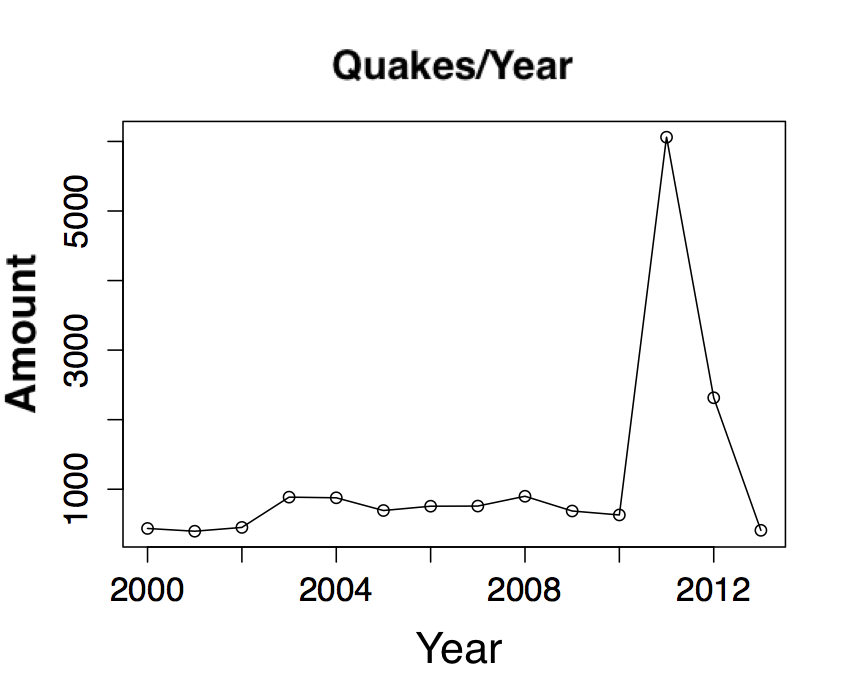
\includegraphics[scale=0.5]{img/ocorrenciasAno.png}
\caption{Amount of earthquake by year.}
\label{ocorrenciasAno}
\end{figure}

Based on the statement done before and considering that we want earthquakes that follow more stable patterns, we selected the ones that happened in land areas or very shallow sea areas, with maximum depth of 100km.

\subsubsection{Regions}
For the experiments, the data was changed into slices for every year. Each slice is as follows: if the base contains data about a time interval of 10 years, it will be split in 10 slices.

We also selected some sub-areas in Japan to better extract and understand earthquakes characteristics and patterns. Those areas are Kanto, Kansai, Touhoku and East Japan. The Figure~\ref{alljapan} shows how we defined them. 

\begin{figure}[H]
	\centering
	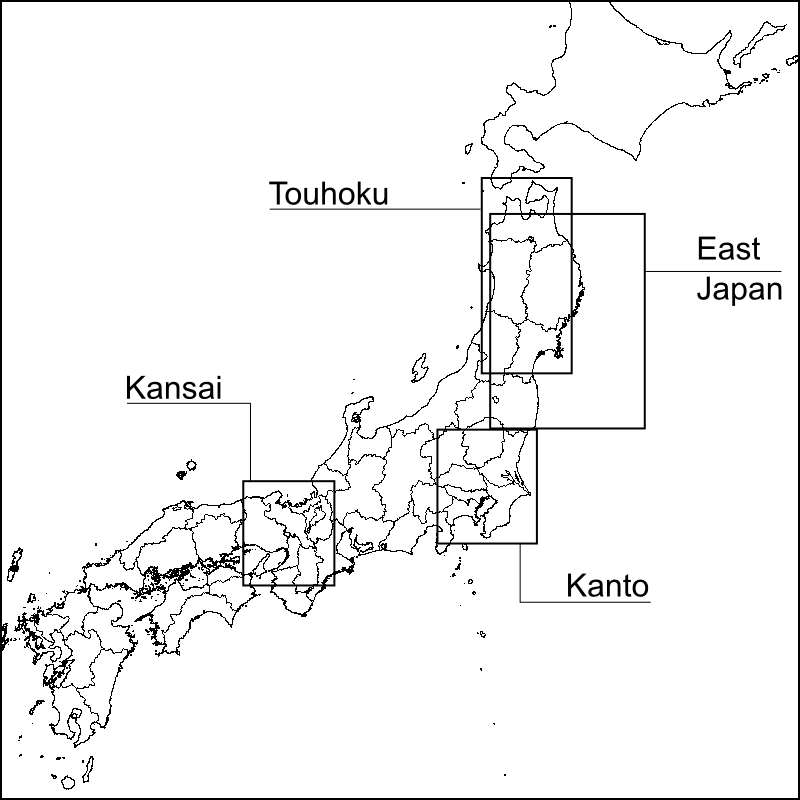
\includegraphics[scale=0.25]{img/alljapan.png}
	\caption{Japan and the areas used in this studied.}
	\label{alljapan}
\end{figure}


They are described as follows:

\paragraph{Kanto} Kanto is the region around Tokyo. It is an area with high seismologic activity during the years we studied. Its coordinates are 34.8 North, 138.8 West, with  2025 bins. Each bin covers an area of approximately 25km$^2$.

\paragraph{Kansai} Kansai is the region that includes Kyoto, Osaka and many others historical cities. In this area, rather than Kanto area, there is a small seismic activity. Its coordinates are 34 North, 134.5 West, with 1600 bins. Each bin covers an area of approximately 25km$^2$.

\paragraph{Touhoku} Touhoku is the region in the North of the main Japanese island. It has some clusters of seismic activities during the years we studied. Its coordinates are 37.8 North, 139.8 West, with  800 bins. Each bin covers an area of approximately 100km$^2$. 

\paragraph{East Japan} Is the region that is related with the east coast of Japan. It is the most different area, because it has earthquakes that happened both in land or in the sea. It was in this region that the 9.0 $M_w$ earthquake happened. Its coordinates are 37 North, 140 West, with 1600 bins. Each bin covers an area of approximately 100km$^2$. 

\subsubsection{Depth Histogram of Earthquakes}


The patterns of earthquakes are dependent of the epicentre. We wanted to explore the relation between the depth of the earthquakes and how would our models behave on those situations.

In Figure~\ref{histogramQuakes}, it is possible to understand that most of the earthquakes happened with depths smaller or equal to 100 km. The earthquakes deeper than 100 km are fewer and more distant, as it is in the same Figure.\\

\begin{figure}[]
	\centering
	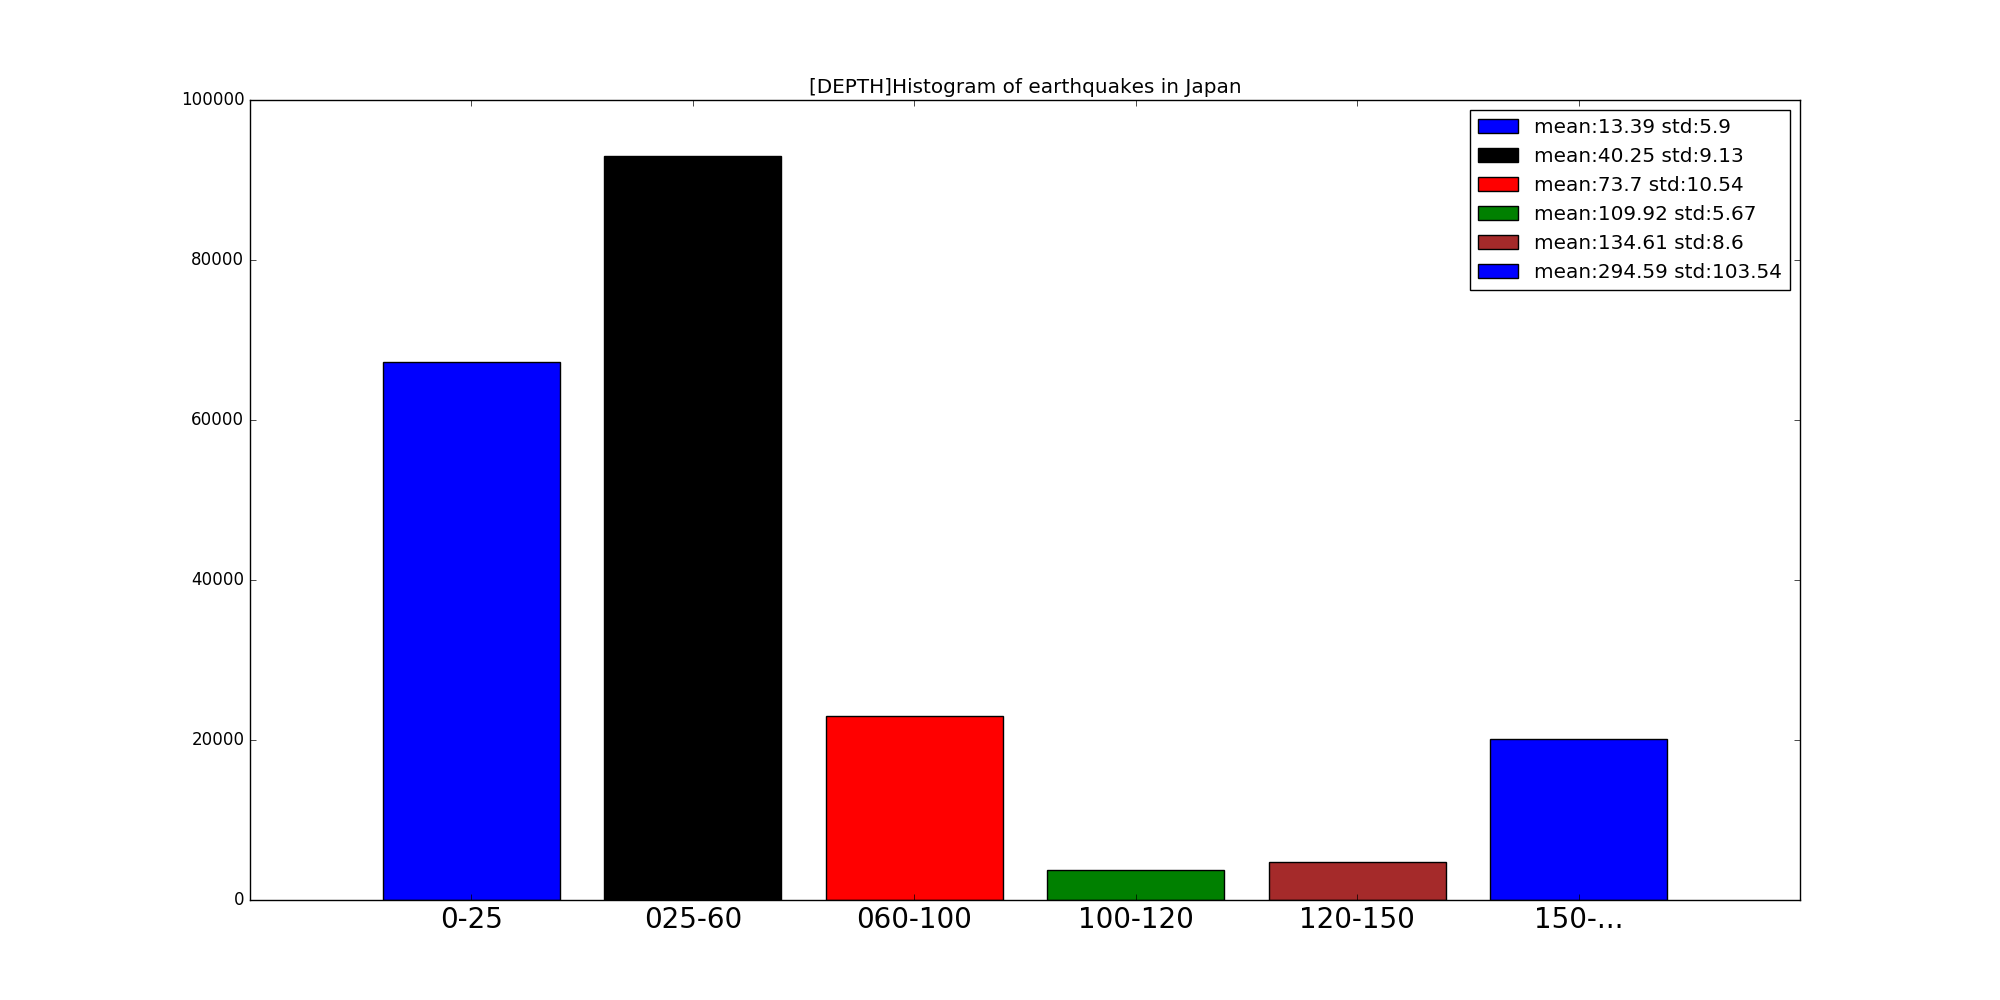
\includegraphics[scale=0.15]{img/detphsNew.png}
	\caption{Depth Histogram of earthquakes.}
	\label{histogramQuakes}
\end{figure}

The reason we decided to groups as: earthquakes with depth until 25 km, until 60 km or until 100 km. This is because shallow earthquakes are considered to be more independent earthquakes~\cite{yamanaka1990scaling}.

\subsubsection{Mainshocks and Aftershocks - Clustering}\label{Clustering}

In the Section~\ref{1year-model}, we explained that we have two kinds of models, the ones that only consider aftershocks and those that consider both mainshocks and aftershocks. Therefore, it is needed to isolate, to classify the earthquakes into one of these two groups.

The question is how should it be done. The simplest way, is to select earthquakes with magnitude above 3.0 in the Richter Scale and then to consider those as the mainshocks. The distribution of earthquakes after this selection is exemplified in the Figure~\ref{quakesKanto}.

\begin{figure}[H]
	\centering
	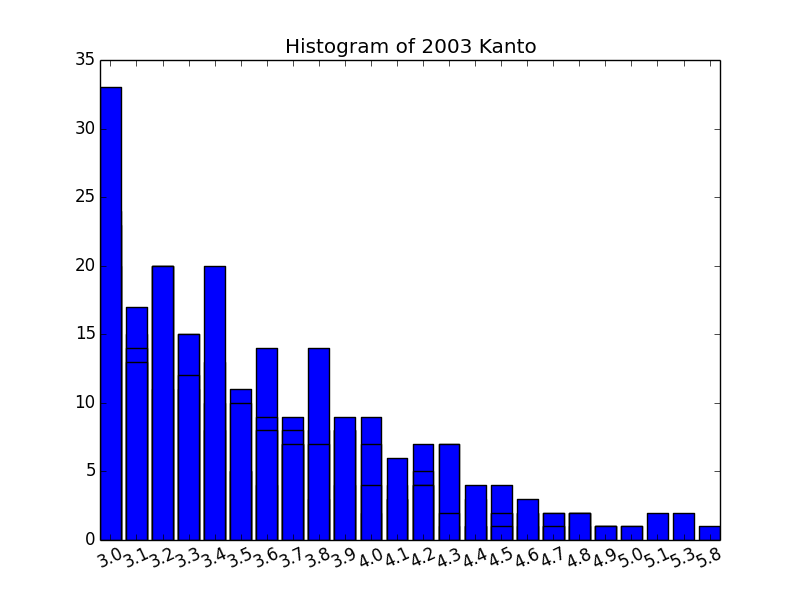
\includegraphics[scale=0.35]{img/Magnitude2003Kanto.png}
	\caption{Histogram of earthquakes stronger than 3.0 in the Richter Scale in Kanto}
	\label{quakesKanto}
\end{figure}

%TODO: check what info I need to use from Gabriel's
The problem with this simple idea is: if a big mainshock happens and it triggers some aftershocks with magnitude higher than 3.0 in the Richter Scale it would be considered as a mainshock. To avoid this problem we used two methods proposed in the literature: Window Methods and the Single-Link Cluster. For more information about these methods, see reference~\cite{van2012seismicity}.

\subsection{Experimental Design}

The first experiment was made to compare the all the models proposed with each other and to discover which method would achieve higher log-likelihood values. We created new scenarios, applying the methods for all regions and for the years of 2005-2010. We also used 3 kinds of catalogues: the JMA and the declustered catalogues form the Window method and the SLC method. Then, we compared the means of the models log-likelihood values using the ANOVA test. If a group of variables considered for the ANOVA test showed no statistically significant difference, we applied the Paired Student t-test, in the case all groups showed statistically significant difference, the Tukey HSD methodology analysis was used.

We also made a magnitude experiment. This experiment was done to explore the influence of the magnitude in all models generated. We split them into slices composed of earthquakes that have magnitude in a given magnitude interval. The we calculated the log-likelihood of these slices and applied the ANOVA test to compared these sliced-models.


\subsubsection{The Mainshock Models and Mainshock with Aftershock Method Experiments}\label{bigExp}
 Here we describe the catalogues and the evolutionary operators used for the experiments. Then we specify the models comparison.
 
\paragraph{The catalogues}\label{catalogs}

The data used was from JMA catalogue, with the minimum magnitude of 3.0 and the two declustered catalogues, obtained from the methods explained in the Section~\ref{Clustering}. The models that use these catalogues have in the word Window appended at their names, for the methods that used the Window declustering, or \textit{SLC}, for the methods that used the Single Link Cluster. 

\subsubsection{Models Comparison}
For this new experiment, we used even more scenarios (space/time regions) than the others. Each scenario contains the earthquakes for the regions of Kanto, Kansai, Touhoku and East Japan for a given year (2005-2010). We wanted to explore if there exists any influence in the performance of the models that are caused by the depth of an earthquake. So, the scenarios are also composed by introducing a three groups depths thresholds. They are: of earthquakes with depth smaller than 25km, or between 0km and 60km or even between 0km and 100km.

These methods are stochastic methods and hence are variations of the GAModel, we decided to maintain the number of repetitions without redoing the Power of the Student t-test.

\subsection{Statistical Analysis of the Results}\label{anova}

The goal is to discover if there is any variation between the methods and which are the most influential variables. For achieve that, we will use the ANOVA test.

In the ANOVA test, of variance of one specific variable with 95\% confidence level, with ``p-value'' < 0.05 it means that there exists a statistical significant evidence that the variables variance are different from.

There are some tests hypothesis for this experiment that we want to analyse. They all can be generalised as follows:

$$\begin{cases} H_0: \text{The population means are equal.} &\\
H_1: \text{The population means are different.}&\\
\end{cases}$$\\

Then, if there is no statistical significant difference between the means, we apply the Tukey HSD. We apply it on the results obtained from the ANOVA test to specify which groups differ. Tukey's methodology analysis shows the means of a case with the means of every other case. Doing so, it identifies differences between means :

$$\begin{cases}
\mu_a-\mu_b, \text{where $\mu_a$ is the mean of the first group}\\
                \text{$\mu_b$ is the mean of the second group.}
\end{cases}$$

In the case where statistical significant difference exists, we
explore this by pairing the measures observations of two
groups.

%~\cite{Campelo2015-01}. -- Nao precisa citar a aula de estatistica
% Em geral, se voce vai citar algo de nivel ``livro texto'', voce tem que ir atras
% da referencia original, e nao citar onde voce viu a referencia sendo usada.

That is:

$$\begin{cases}
H_0: \mu = 0, \text{the difference between observations is 0.}&\\
H_1: \mu != 0, \text{difference between observations is not 0.}
\end{cases}$$\\

%%% trabalho 19.07 começa aqui
\subsubsection{Results from The Mainshock Models Mainshock with Aftershock Models Experiment}\label{resultsBigExp}

An one-way between subjects ANOVA was conducted to compare the effects of the models, the years and regions on the log-likelihood value. In this study there are the models: \textit{ReducedGAModel}, \textit{Emp-ReducedGAModelSLC}, \textit{Emp-GAModel}, \textit{Emp-ReducedGAModel}, \textit{GAModelWindow}, \textit{ReducedGAModelWindow}, \textit{GAModelSLC}, \textit{ReducedGAModelSLC}, \textit{Emp-GAModelWindow}, \textit{Emp-ReducedGAModelWindow}, \textit{GAModel} and \textit{Emp-GAModelSLC}.

Based on the results of this first test, it is evident that all variables are significantly different. The results of the experiments are in the Table~\ref{anovatest1}. For all,the confidence level is set to 95\% .

%TODO: pegar monografia e ver o que eu tinha pensado
\begin{table*}[!htb]
	\centering
	\begin{tabular}{|l|l|l|l|l|l|}
		\hline
		{Variable} & {Degrees of Freedom} & {Sum Sq}    & {Mean Sq}   & {F Value} & {Pr(\textgreater F)} \\
		\hline
		Model    & 15           	  & 149303768  & 9953585   & 63.72    & \textless2e-16     \\
		\hline
		Year     & 5                  & 414016420  & 82803284  & 530.06   & \textless2e-16     \\
		\hline
		Region   & 3                  & 869821655  & 289940552  & 1856.02   & \textless2e-16	\\    
		\hline
	\end{tabular}
	\caption{ANOVA Test Results Values - Mainshock Models Mainshock and Aftershock Models.}
	\label{anovatest1}
\end{table*}

Because we found statistically significant result, we applied a Post-hoc comparisons using the Tukey HSD analysis methodology. It compared each condition with all others. For example, it compares the values from the GAModel with the GAModelWindow. It indicated that the models Emp-ReducedGAModelWindow, GAModelWindow, ReducedGAModelWindow, GAModelSLC, ReducedGAModelSLC achieve statistically better or equal results in terms of log-likelihood when compared with the other models and when compared with themselves, they are statistically similar. The results of the experiments are in the Table~\ref{anovatest2}. For all, again,the confidence level is set to 95\% .
     
\begin{table*}[!htb]
	\centering
	\begin{tabular}{|l|l|l|l|l|l|}
		\hline
		{Variable} & {Degrees of Freedom} & {Sum Sq}    & {Mean Sq}   & {F Value} & {Pr(\textgreater F)} \\
		\hline
		Model    & 4           	  & 884882  & 221220   & 1.604    & 0.171    \\
		\hline
		Year     & 5                 & 150297410  & 30059482  & 217.955   & \textless2e-16     \\
		\hline
		Region   & 3                  & 234225270  & 78075090  & 566.107   & \textless2e-16	\\    
		\hline
	\end{tabular}
	\caption{ANOVA Test Results Values - Emp-ReducedGAModelWindow, GAModelWindow, ReducedGAModelWindow, GAModelSLC, ReducedGAModelSLC.}
	\label{anovatest2}
\end{table*}

Therefore, to confirm that statistically the models are similar, we applied the conducted the ANOVA test considering only with the models indicated by the Tukey HSD, see Figure~\ref{modelANOVA-100and5}.

\begin{figure}[H]
	\centering
	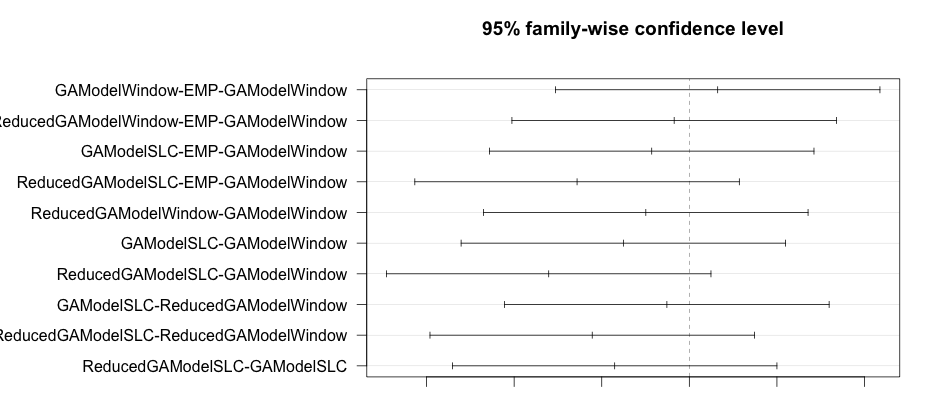
\includegraphics[scale=0.28]{img/modelANOVA-100and5.png}
	\caption{Intervals of Confidence 95\% of differences between the Mainshock Models Mainshock and the Aftershock Models, taken two by two.}
		\label{modelANOVA-100and5}
\end{figure}

This time, we found statistically significant difference only for the year and region condition. To show that the models results are not statistically different from each other, we applied a pairing analysis.

From the the pairing analysis, we decided to use the \textit{ReducedGAModelSLC} as the representative method of this study. That is because, in most cases when its values were compared, it showed a little better performance in the means of the log-likelihood values. For the results, see the Table~\ref{Paired}.

In this Table, the column labelled $\mu_a - \mu_b$ shows the result of paired difference between the models referred in the ``Models Compared'' column. The p-value shows the significance value of the paired {\it Student's t-test} for the null hypothesis `` The paired difference of the means of the models is equal''.


\begin{table*}[!htb]
	\begin{center}
		\begin{tabular}{|c|c|c|c|}
			\hline
			\multicolumn{1}{|c|}{Region} &
			\multicolumn{1}{|c|}{Models Compared} & \multicolumn{1}{|c|}{Mean of $\mu_a - \mu_b$}&
			\multicolumn{1}{|c|}{p-value} \\
			\hline
			
			Kansai & EMP-\textbf{GAModelWindow} - GAModelWindow &
			 38.67553 &  3.304e-05 \\
			
		    & EMP-\textbf{GAModelWindow} - ReducedGAModelWindow & 4.272185  & 0.2607\\
			
			& EMP-\textbf{GAModelWindow} - GAModelSLC & 
			112.0424 &  1.122e-05\\

			&EMP-GAModelWindow - \textbf{ReducedGAModelSLC} &  
			-1.787262 & 0.5673 \\
			
			& GAModelWindow - \textbf{ReducedGAModelWindow} &
			-34.40335 & 0.000963\\
			
			& \textbf{GAModelWindow} - GAModelSLC &
			 73.36687  &9.065e-06\\
				
			& GAModelWindow - \textbf{ReducedGAModelSLC} &
			-40.46279 & 6.32e-05\\
				
			& \textbf{ReducedGAModelWindow} - GAModelSLC &
			107.7702  & 2.632e-05\\

			& ReducedGAModelWindow - \textbf{ReducedGAModelSLC} &
			-6.059447 &0.2982\\

			& GAModelSLC - \textbf{ReducedGAModelSLC} &
			-113.8297 & 1.2e-05\\

			\hline
			Touhoku & EMP-\textbf{GAModelWindow} - GAModelWindow &
			3.34556 & 0.546\\
			& EMP-\textbf{GAModelWindow} - ReducedGAModelWindow &
			81.60965 & 5.225e-07\\
			&	EMP-\textbf{GAModelWindow} - GAModelSLC &
			63.02216 &0.01971\\
			& EMP-GAModelWindow - \textbf{ReducedGAModelSLC} &
			-62.70586 & 0.007075\\
			& \textbf{GAModelWindow} - ReducedGAModelWindow & 
			78.26409 & 2.938e-05\\
			& \textbf{GAModelWindow} - GAModelSLC &
			59.6766 & 0.04829\\
			& GAModelWindow - \textbf{ReducedGAModelSLC} &
			-66.05142 &0.001231\\
			& ReducedGAModelWindow - \textbf{GAModelSLC} &
			-18.58749 & 0.3443\\
			& ReducedGAModelWindow - \textbf{ReducedGAModelSLC} &
			-144.3155 & 0.000214\\
			& GAModelSLC - \textbf{ReducedGAModelSLC} &
			-125.728 &0.01216\\

			
			\hline
			East Japan & \textbf{EMP-GAModelWindow} - GAModelWindow &
			1.872764  & 0.9539\\

			& EMP-\textbf{GAModelWindow} - ReducedGAModelWindow &
			194.4944 & 1.834e-06\\
			& EMP-\textbf{GAModelWindow} - GAModelSLC &
			189.1155 & 0.0003456\\
			& EMP-GAModelWindow - \textbf{ReducedGAModelSLC} &
			-274.9858 & 4.961e-05\\
			& \textbf{GAModelWindow} - ReducedGAModelWindow &
			192.6217 & 0.003738\\
			& \textbf{GAModelWindow} - GAModelSLC &
			187.2428 &9.495e-06\\
			& GAModelWindow - \textbf{ReducedGAModelSLC} &
			-276.8586 & 4.636e-05\\
			& ReducedGAModelWindow - \textbf{GAModelSLC} & 
			-5.378912 & 0.8576\\
			& ReducedGAModelWindow - \textbf{ReducedGAModelSLC} &
			-469.4803 & 1.446e-05\\
			& GAModelSLC - \textbf{ReducedGAModelSLC} &
			-464.1014  & 2.38e-06\\

			
			\hline
			Kanto & EMP-\textbf{GAModelWindow} - GAModelWindow &
			57.95612 & p-value = 0.00138\\
			& EMP-\textbf{GAModelWindow} - ReducedGAModelWindow &
			79.60781 & 3.441e-05\\
			& EMP-\textbf{GAModelWindow} - GAModelSLC &
			274.3114  & 5.717e-06\\
			& EMP-GAModelWindow - \textbf{ReducedGAModelSLC} & 
			-96.61803  & 6.22e-07\\
			& \textbf{GAModelWindow} - ReducedGAModelWindow & 
			21.65169  & 0.1105\\
			&\textbf{GAModelWindow} - GAModelSLC &
			216.3553  & 2.302e-07\\
			& GAModelWindow - \textbf{ReducedGAModelSLC} &
			-154.5741  & 1.741e-05\\
			& \textbf{ReducedGAModelWindow} - GAModelSLC &
			194.7036  & 3.678e-05\\
			& ReducedGAModelWindow -\textbf{ReducedGAModelSLC} &
			-176.2258 & 4.337e-06\\
			& GAModelSLC - \textbf{ReducedGAModelSLC} &
			-370.9294 &1.942e-06\\
			\hline
		\end{tabular}
	\end{center}
	\caption{Paired Experiment Result.}
	\label{Paired}
\end{table*}



%TODO: add only the real and the best model figures
\subsection{The Models Examples And The Real Data}

The Figure~\ref{gamodel2005eastjapan} shows a model from the GAModel method for the year 2005 in East Japan. The next Figure,~\ref{reduced2005eastjapan} shows a model from the ReducedGAModel~\ref{reducedGAModel} method for the year 2005 in East Japan.

All Figures,~\ref{gamodel2005eastjapan}~\ref{reduced2005eastjapan}~\ref{hybridgamodel2005eastjapan}~\ref{hybridreduced2005eastjapan},  indicate a low earthquake intensity as white while the more intensity areas, are shown in red. They are, in order, the data visualisation for the model from: the GAModel, the ReducedGAModel, the Emp-GAModel and the Emp-ReducedGAModel for East Japan in 2005. The Figure~\ref{real2005eastjapan} represents the earthquake occurrences in the same region and year.


%\begin{figure}[H]
%	\centering
%	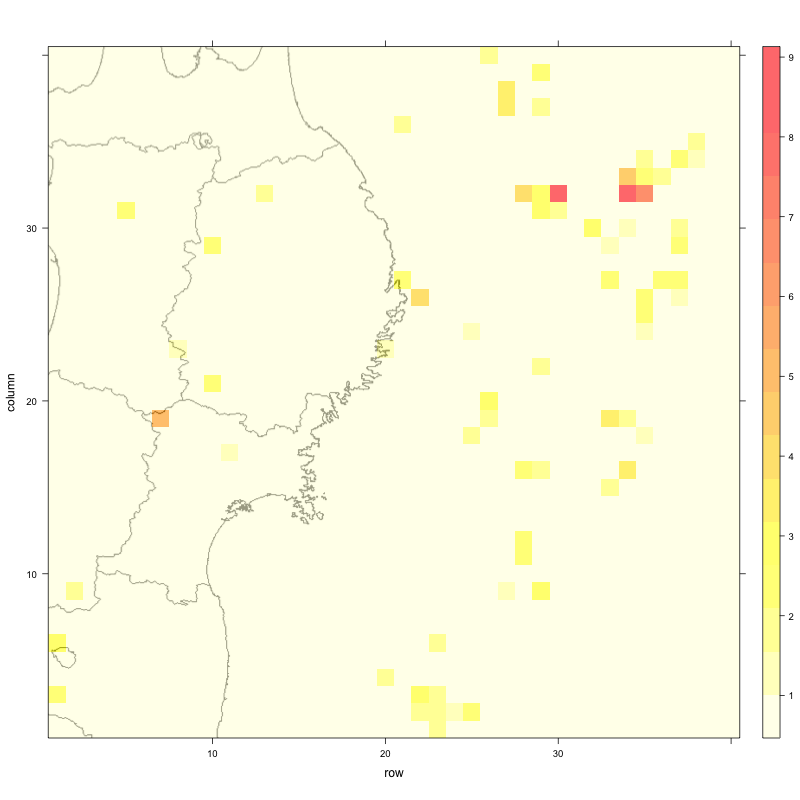
\includegraphics[scale=0.2]{img/gamodel2005eastjapan.png}
%	\label{gamodel2005eastjapan}
%\end{figure}
%
%
%\begin{figure}[H]
%	\centering
%	\begin{minipage}{0.45\textwidth}
%		\centering
%		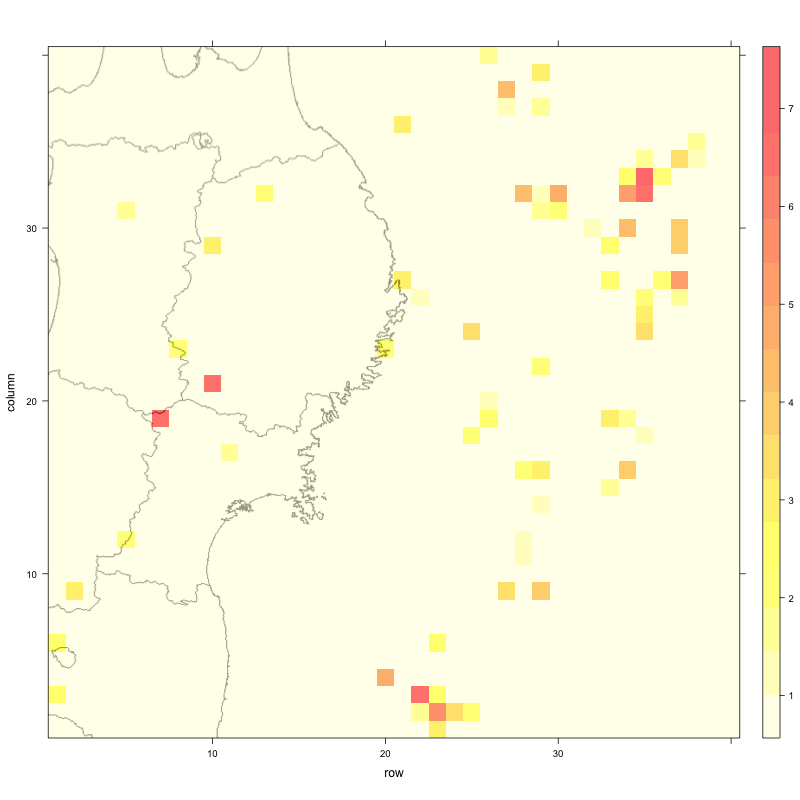
\includegraphics[scale=0.2]{img/reduced2005eastjapan.png}
%		\label{reduced2005eastjapan}
%	\end{minipage}
%	\begin{minipage}{0.45\textwidth}
%		\centering
%		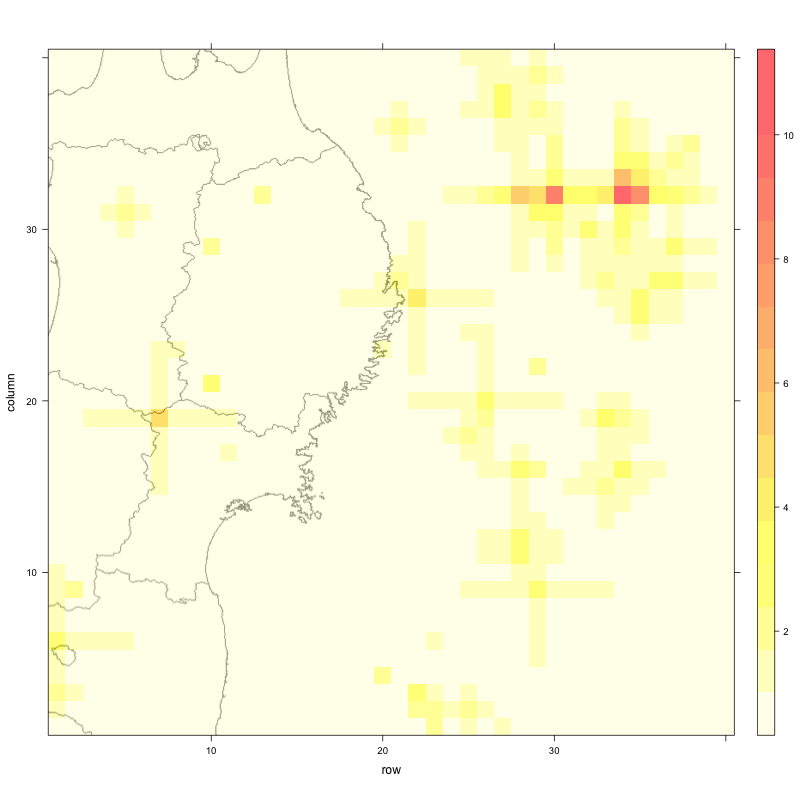
\includegraphics[scale=0.2]{img/hybridgamodel2005eastjapan.png}
%		\label{hybridgamodel2005eastjapan}
%	\end{minipage}
%	\caption{The Figure on the left is the ReducedGAModel model for the year of 2005, East Japan, and the one on the right Emp-GAModel model for the year of 2005, East Japan.}
%\end{figure}
%
%\begin{figure}[H]
%	\begin{minipage}{0.45\textwidth}
%		\centering
%		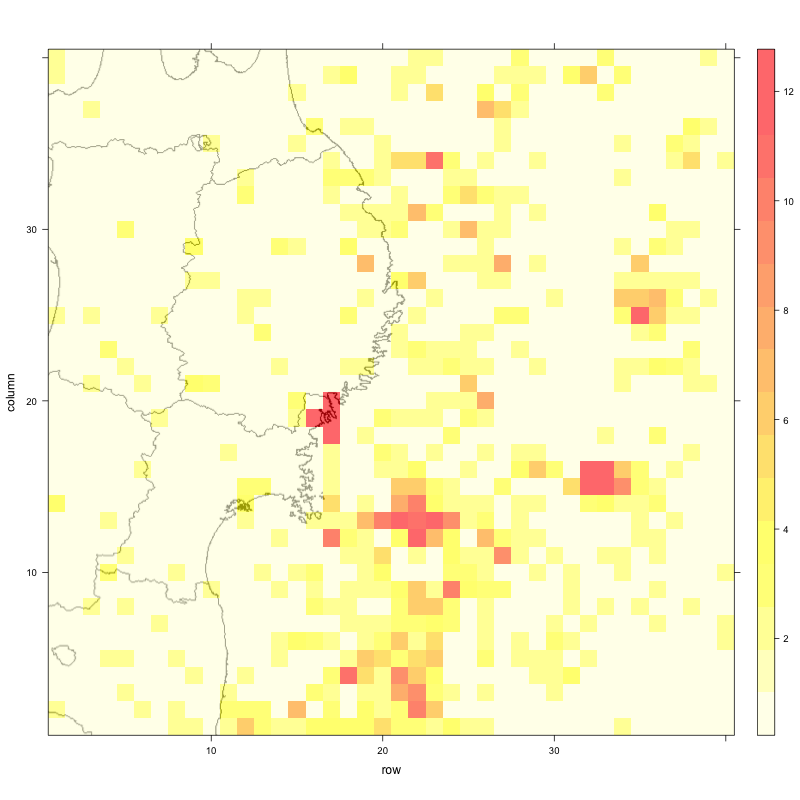
\includegraphics[scale=0.2]{img/real2005eastjapan.png}
%		\caption{Earthquake occurrences in the year of 2005 in East Japan.}
%		\label{real2005eastjapan}
%	\end{minipage}
%	\begin{minipage}{0.45\textwidth}
%		\centering
%		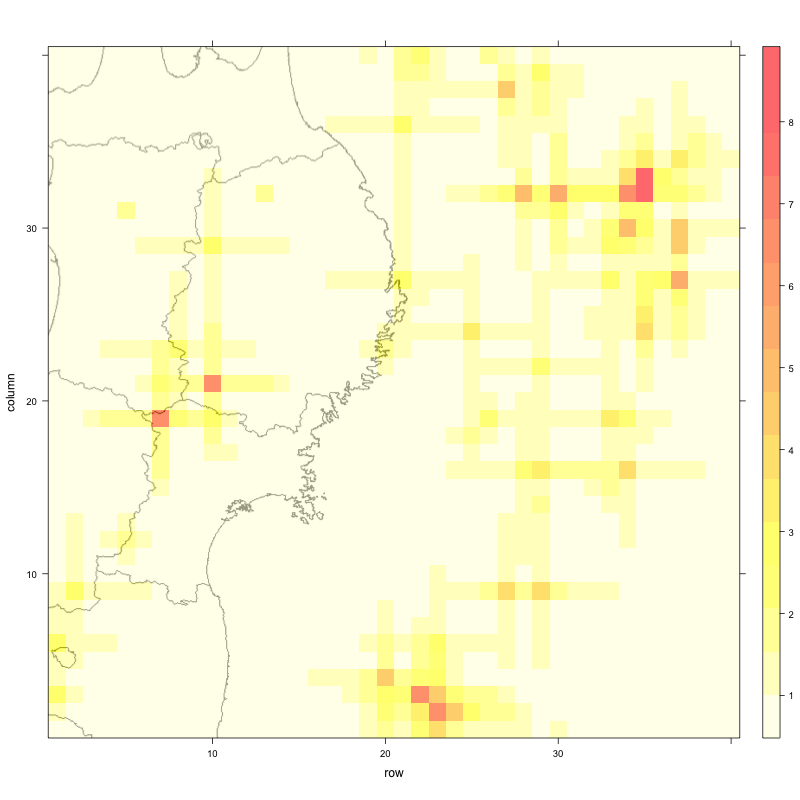
\includegraphics[scale=0.2]{img/hybridreduced2005eastjapan.png}
%		\label{hybridreduced2005eastjapan}
%	\end{minipage}
%	\caption{The Figure on the left is the Emp-ReducedGAModel model for the year of 2005, East Japan, and the one on the right GAModel model for the year of 2005, East Japan, East Japan.}
%\end{figure}




\subsection{Magnitude Experiment}\label{magExp}

In this experiment, we focused on studying how the magnitude of an earthquake affects the model quality, because the patterns of the earthquakes are depended of its magnitude. We wanted to explore the relation between the magnitude of the earthquakes and how would the models behave on those situations.

For that, we created magnitude intervals, where each interval is named as a slice. A slice is an closed interval of 1.0 degree  starting from 3.0 degrees of magnitude, see Section~\ref{catalogs}, and ending in 10.0 degrees. For example, $[3.0-4.0]$ or $[7.0-8.0]$ are two different slices. For each model, we selected only the earthquakes that belong to a slice. Then, we calculate the log-likelihood value.
\subsubsection{Magnitude Study}
From the results already obtain and showed in the section~\ref{resultsBigExp}, when selected the models with earthquakes with depth smaller or equal to 25 km and then we split the models in magnitude intervals, as defined in~\ref{magExp}.

After that, we compared those split models against themselves. Based on the results of this test, it is evident that all variables are still significantly different. The results of the experiments are in the Table~\ref{anovatestMag}. For all, as before, we choose the confidence level to be 95\%.


\begin{table*}[!ht]
	\centering
	\begin{tabular}{|l|l|l|l|l|l|}
		\hline
		{Variable} & {Degrees of Freedom} & {Sum Sq}    & {Mean Sq}   & {F Value} & {Pr(\textgreater F)} \\
		\hline
		Model       & 5            	  & 2.360e+09      & 4.720e+08     & 2828     & \textless2e-16     \\
		\hline
		Year        & 3                  & 4.624e+09   & 1.541e+09    & 9234     & \textless2e-16     \\
		\hline
		Magnitude   & 7                  & 3.726e+09   & 5.322e+08    & 3189     & \textless2e-16	\\    
		\hline
	\end{tabular}
	\caption{ANOVA Test Results Values - Magnitude Study.}
	\label{anovatestMag}
\end{table*}

We found statistically significant result and, as before, we applied the Tukey HSD test. The results are shown in Figure~\ref{modelANOVAMag} and the \textit{NULL} field was used as the model with all magnitude intervals (the complete model).

It indicated that the interval $[3.0-4.0]$ always performed, in terms of log-likelihood values, worse than all other intervals. this phenomenon also happens in the interval $[4.0-5.0]$, though in this case, the difference is not as big as the last one. The other intervals show no significant difference.
From the results found, we decided to chose only earthquakes with magnitude higher than 4.0 as our threshold value.

%\begin{figure}[H]
%	\centering
%	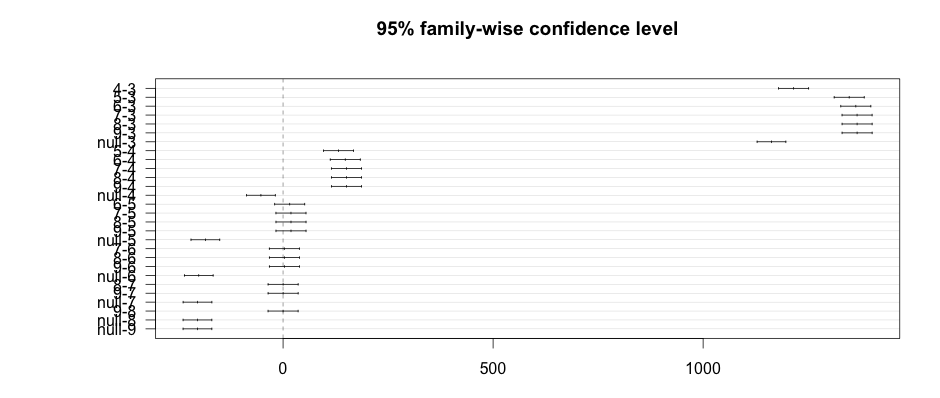
\includegraphics[width=9cm,height=9cm,keepaspectratio]{img/magModels.png}
%	\caption{ANOVA results - Models from Magnitude Study.}
%	\label{modelANOVAMag}
%\end{figure}
%%% trabalho 19.07 termina aqui
\subsubsection{Catalogues and Models }
This experiment used the same catalogues used in the previous experiment~\ref{bigExp}. 

The models also are the models from the last experiment. We also created the new models, considering the slices and add them to the comparison. That lead to a comparison with the models from the last experiment and the models sliced.


\subsubsection{Statistical Analysis}
The goal is to discover if the magnitude influences any variation in the methods and how it does.

For this experiment, we followed the same design from the Section~\ref{anova}.

\subsubsection{Results}\label{Results}




%TODO: add future work with Gabriels
%TODO: this section should be a revision of all
\section{Conclusions}\label{Conclusions}
%\end{document}  % This is where a 'short' article might terminate

%ACKNOWLEDGMENTS are optional
\section*{Acknowledgments}
The authors would like to thank Bogdan M. Enescu, from the department
of Earth Evolution Sciences in the university of Tsukuba for his
useful comments. 

We would also like to thank the Japan Meteorological Agency for the
earthquake catalog used in this study.
